\chapter{Evaluation}
\label{ch:eval}

%TODO: resource trebovaniya

\section{The \texttt{PorthosC} in work}

\subsection{The X-graph compilation}

As a simple example of the compilation process discussed in Section~\ref{ch:impl:proc:x-compiler:compilation}, consider the tiny C test in Figure~\ref{ex:compilation}.
This function does not perform any useful computation, however it contains several syntactic elements (such as prefix increment or loop-breaking statements), which are supported by \porthos[2] comparing to its predecessor.
The control-flow subgraph \xgraph[CF] of the non-unrolled event-flow graph is presented on the right-hand side of the Figure (all graphs generated by \porthos[2] are produced with the help of the open-source library \texttt{Graphviz}~\cite{ellson2001graphviz}).

Each event of the control-flow graph contains the unique number (generated by the \texttt{hashCode} method) in curly brackets below the value, which is necessary for correct displaying the graph.
Write events are denoted with the left-directed arrow `\lstinline{<-}', and the functions \lstinline{load} and \lstinline{store} denote the type of the shared memory event.
The primary transitions that denote unconditional jumps or if-true-transitions are pictured with solid lines, and the alternative transitions that denote if-false-transitions are pictured with dotted lines.
The graph contains a single source event and a single sink event (represented by the grey triangles).

\begin{figure}[!h]
\begin{minipage}{.4\textwidth}
\begin{lstlisting}[language=Java,basicstyle=\ttfamily\small]
void test(int &x, int &y) {
    int r;
    while ((5 + 4/2 * x) 3 
      == 1) {
        if (y > 6)
            continue;
        else if (++y > 7) {
            r = r + 10;
            break;
        }
        r = 11;
    }
    y = x + 1;
}
\end{lstlisting}
\end{minipage}
%
\begin{minipage}{.59\textwidth}
  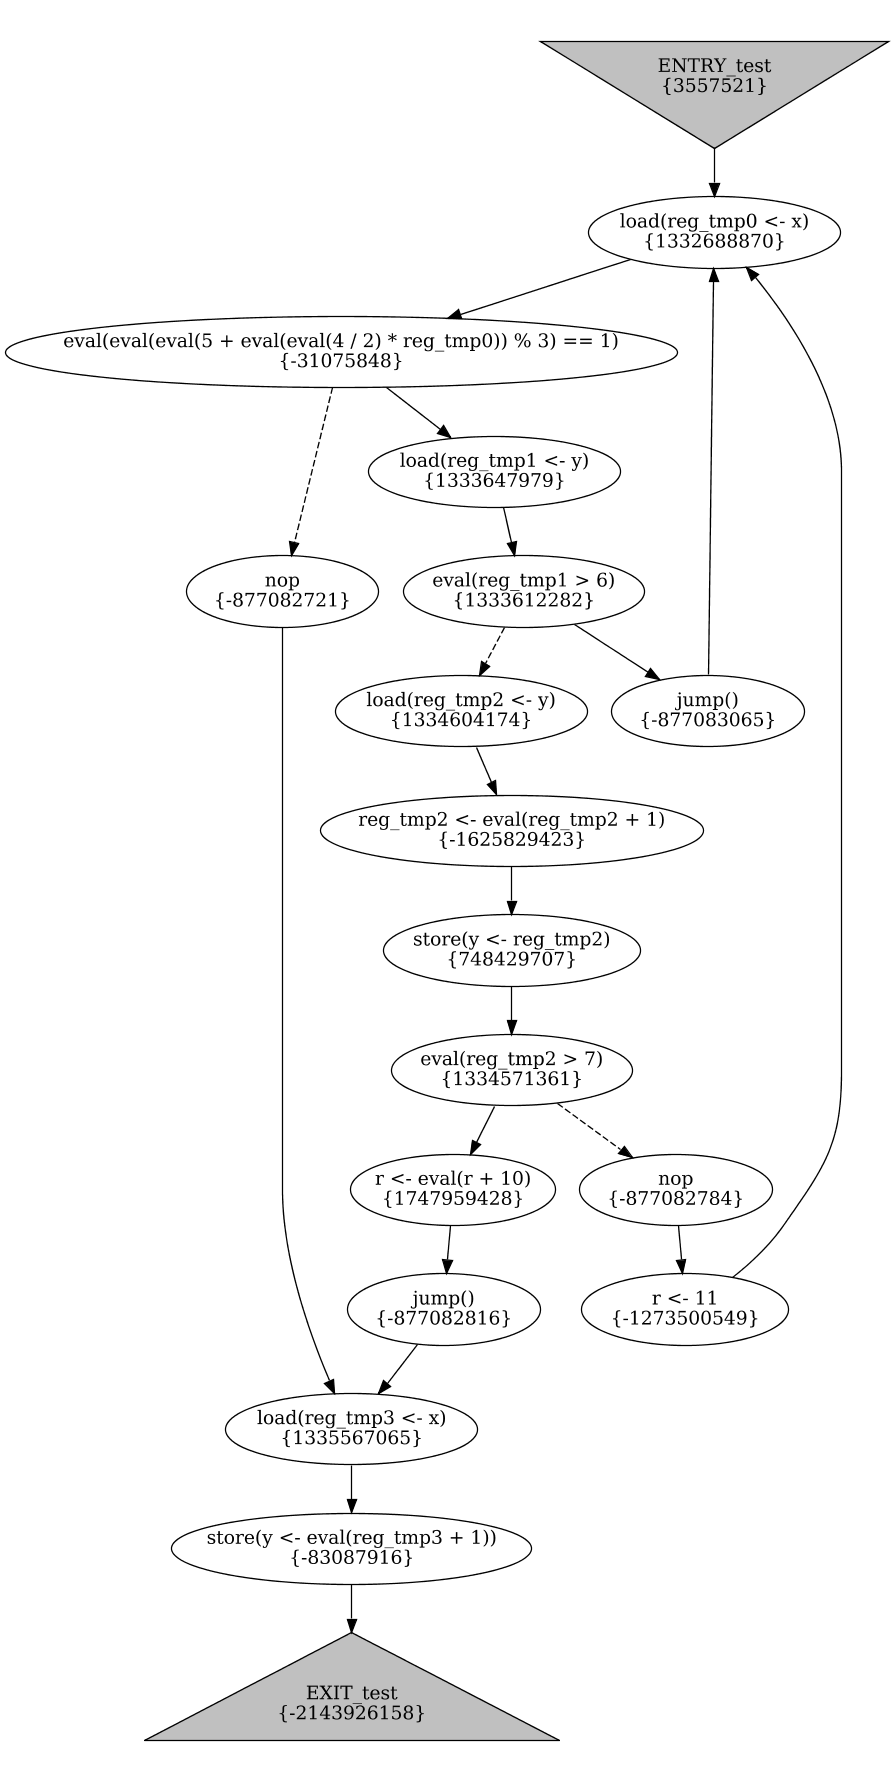
\includegraphics[width=\textwidth,keepaspectratio]{img/my/graphs/test.png}
\end{minipage}
%
\caption{An example of a C function compiled to the event-flow graph}
\label{ex:compilation}
\end{figure}

The arguments \lstinline{x} and \lstinline{y} of the function are passed by reference, therefore they are treated as global variables.
The local variable declaration `\lstinline{int r;}' produces no events (it is processed by the X-graph pre-compiler that invokes the memory manager to create the new local variable \lstinline{r}).

The first event `\lstinline{load(reg_tmp0 <- x}' loads the value of the global variable \lstinline{x} into the temp register \lstinline{reg_tmp0} in order to satisfy the requirement that all computation must be performed over local variables;
note that each element of the computational tree `\lstinline{eval(eval(eval(5 + eval(eval(4 / 2) * reg_tmp0)) % 3) == 1)}' is represented by a local memory unit (either \texttt{XComputationEvent} or \texttt{XConstant} or \texttt{XRegister}).
The node of this computational event in the control-flow graph has two outgoing edges, the primary edge to the `\lstinline{load(reg_tmp1 <- y}', the first event of the then-branch of the while-loop, and the alternative edge to the \lstinline{nop}-event representing the only event of the else-branch.

As is was discussed in Section~\ref{ch:impl:model:xgraph}, all computation events have no impact to the global state of the concurrent system.
Therefore, the interpreter does not \textit{emit} computational events, but it \textit{creates} them.
This means, when the \texttt{Y2XConverterVisitor} processes the expression tree `\lstinline{(5 + 4/2 * x) 3 == 1}', it calls the method \texttt{createComputationEvent} of the interpreter that only creates the computation event and does not change its state.
However, once the converter meets the global variable \lstinline{x}, it calls the interpreter method \texttt{emitMemoryEvent} to copy its value to a temp register; since it meets the global variables involved to the computation before it ends to process the whole computation expression, the values of all these global variables will be copied to temp registers \textit{before} the computation expression is used by any other event.
Note that if the computation expression has not been used by any other event (for example, as the constant \lstinline{1} in the following C code: `\lstinline{foo(); 1; bar();}'), it is lost from the model (by the term \textit{use} here we mean that the computation event is evaluated as a guard or assigned to another memory unit).


\subsection{The X-graph unrolling}

Once the \xgraph[CF] is constructed, it should be unrolled to an acyclic flow-graph (as it was discussed in Section~\ref{ch:impl:proc:x-unroll}).
The Figure~\ref{ex:unrolling} shows the control-flow subgraph \xgraphU{CF} of the event-flow graph from the previous example (see Figure~\ref{ex:compilation}) unrolled up to bound $k=16$.
The labels of events in the picture are augmented by the event reference-id number (the unrolling depth), separated from the event value by the comma.

Note that the graph does not become a tree after removing the sink node.
Some branches of the graph are merged when the executions have the same event with the same unrolling depth number.
For example, primary transitions of both events `\lstinline{[r <- 11, 10]}' and `\lstinline{[jump(), 10]}' (produced by executions of the first iteration of the \texttt{while} loop) lead to the same event `\lstinline{[load(reg_tmp0 <- x), 11]}' (the first event of the second loop iteration).

%(said before in 4_impl:unrolling)
%Also note that comparing to the unrolling bound description given in Section~\ref{ch:impl:proc:x-unroll}, 
%As the distinction between complete and incomplete sink nodes is not implemented yet, 

\begin{figure}[!h]
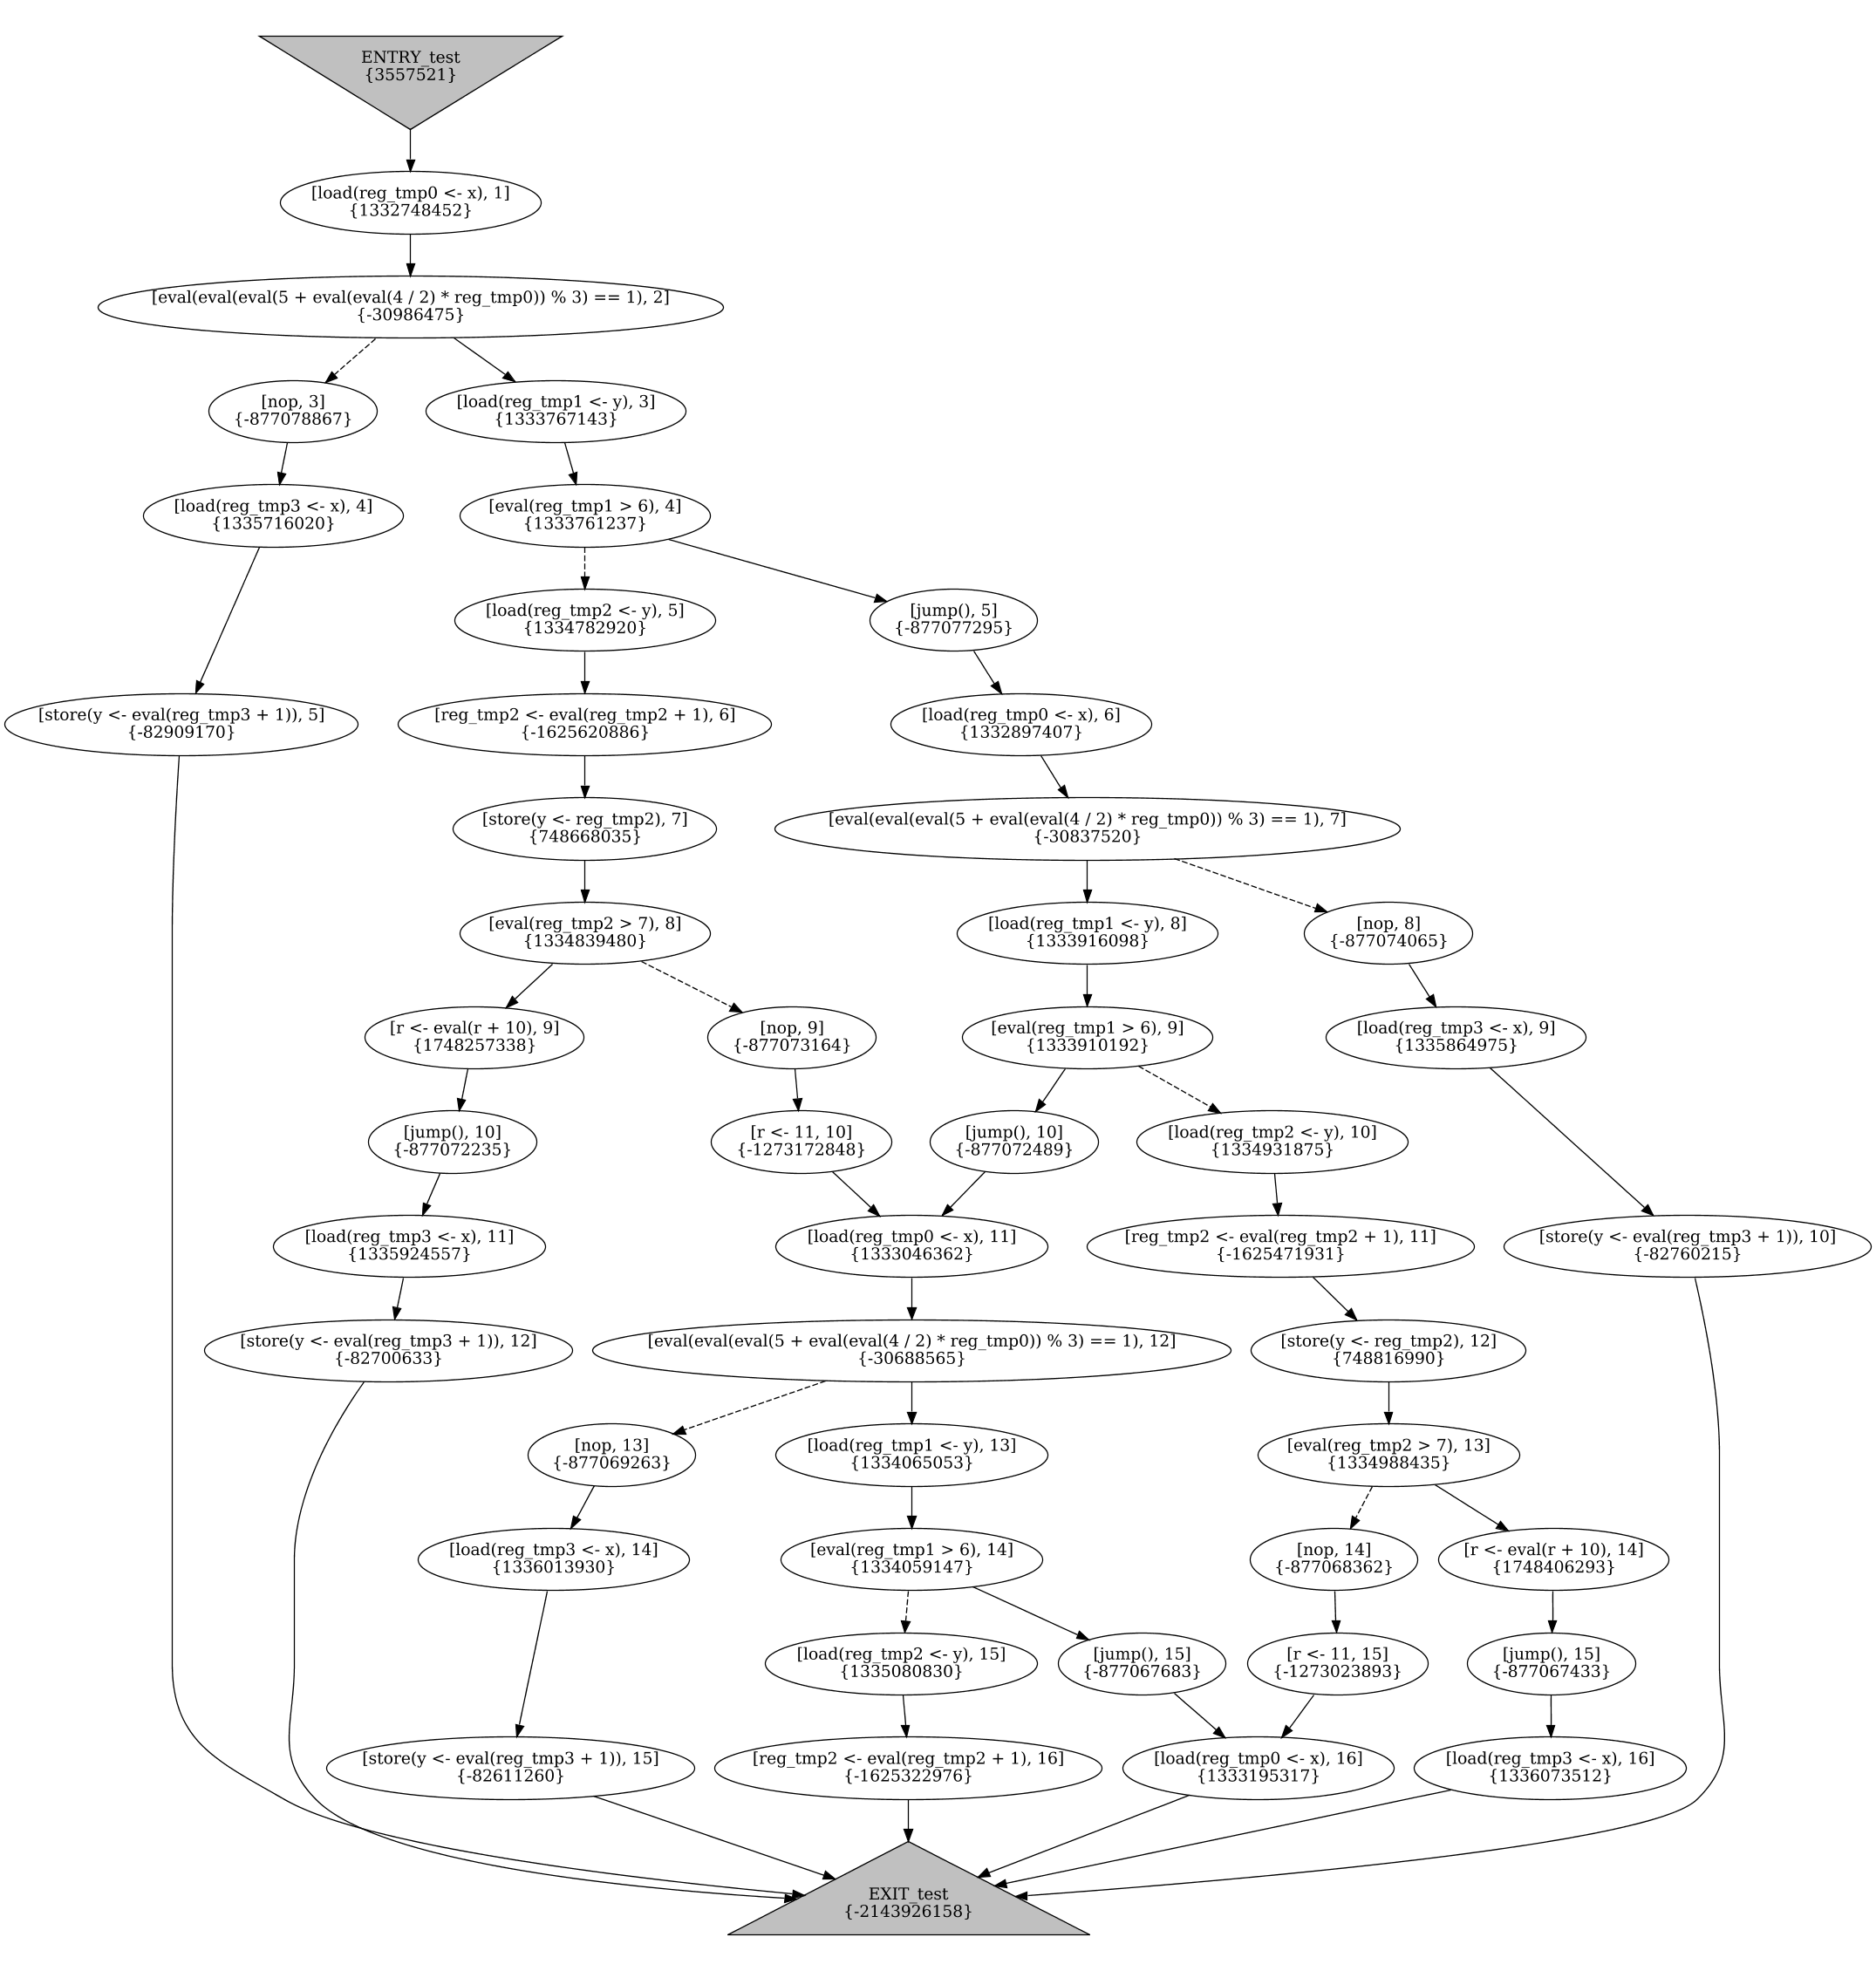
\includegraphics[width=\textwidth,keepaspectratio]{img/my/graphs/test_unrolled.png}
\caption{Unrolling of the event-flow graph presented in Figure~\ref{ex:compilation}}
\label{ex:unrolling}
\end{figure}


\section{Performance}

\subsection{State reachability analysis}

As an example of the C program liable for the reachability and portability analysis, consider the Dekker's algorithm for mutual exclusion of two processes, originally described by Dijkstra~\cite{dijkstra1962over}; the program is presented in Appendix~\ref{apx:dekker}.

For checking the reachability of the final state of the last states (sink events) of unrolled graphs compiled for a certain hardware architecture, \porthos[2] encodes both program and hardware memory model constraints as it was discussed in Section~\ref{ch:enc:bmc}.
%The result formula is then solved by the Z3 

%TO-DO: fix interface
%To run \porthos[2] in reachability analysis mode, we use the command `\lstinline{mousquetaires.DartagnanApp -i benchmarks/litmus_C11/Dekker.c -s tso}'

The standard output of the tool looks as following:
\begin{lstlisting}
$ java Dartagnan -i benchmarks/C11/Dekker.c -s tso
Interpreting...
Unrolling...
Program encoding...
Memory model encoding...
#=59
Solving...
{
  "result": "NonReachable",
  "interpretationTimer": {
    "elapsedTimeSec": 0.134
  },
  "unrollingTimer": {
    "elapsedTimeSec": 0.031
  },
  "programEncodingTimer": {
    "elapsedTimeSec": 0.14
  },
  "memoryModelEncodingTimer": {
    "elapsedTimeSec": 2.984
  },
  "solvingTimer": {
    "elapsedTimeSec": 0.037
  },
  "errors": []
}
\end{lstlisting}

For time benchmarking we ran the tool 5 times and computed the median of the encoding time.
Benchmarking was performed on the Linux machine 8-core Intel(R) Core(TM) i7-3632QM CPU @ 2.20GHz, Java(TM) SE Runtime Environment (build 1.8.0\_161-b12) (Java virtual machine was configured by default parameters).
The time was measured by the tool itself via the Java method \texttt{System.currentTimeMillis}.
For \porthos[1] we specify the unrolling bound $k_1 = 2$ (which means that all loops are executed twice), and for \porthos[2] we specify the bound $k_2 = 32$ (which means approximately the same, because

\porthos[2] shows the full encoding time for the Dekker's algorithm 2.699 sec (from which 0.152 sec spent for the program encoding, and other part spent for the memory model encoding).
In contrast, \porthos[1] shows the encoding time 6.152 sec (from which 0.223 sec spent for the program encoding). %, which is considerably better result.
Thus, the performance of the encoding stage has been improved \textbf{in 2.7 times}.

As the time spent for the interpretation and unrolling stages is negligible comparing to the encoding time, we conclude that the new architecture implies minor performance overhead comparing to the previous version of the tool.
The time spent by the SMT solver while considering the SMT formula encoded by \porthos[2] was 0.039 sec, and in case of \porthos[1] the time was 1.291 sec.
The number of events in the event-flow graph of \porthos[2] is 82 events (among them 59 memory events), and the number of events encoded by \porthos[1] is 95 (among them 51 memory events).
Even though the number of memory events processed by \porthos[1] was less, the time of solving the result SMT-formula was significantly more.
We consider this improvement to be the result of technical optimisations applied to \porthos[2].
The optimisations include:
\begin{itemize}
\item \textit{Memoisation} of the frequently requested calls. \\
    For example, the code of \porthos[1] contains 39 calls that take the subset of a set of events. The pattern is the following: `\lstinline{program.getEvents().stream().filter(e -> e instanceof MemEvent || e instanceof Local).collect(Collectors.toSet())}', \\
    10 of them are performed in a loop over all events (in \texttt{Domain.encode} method of \porthos[2]).
    These calls were replaced by the lazily initialisable memoising methods of \texttt{XProgram}: \\
\begin{lstlisting}[language=Java]
public ImmutableSet<XMemoryEvent> getMemoryEvents() {
    return memoryEvents != null
            ? memoryEvents
            : (memoryEvents = getAllNodesExceptSource(XMemoryEvent.class));
}
\end{lstlisting}
\item Usage of \textit{immutable data structures} (as it was discussed in Chapter~\ref{ch:impl}).
\end{itemize}

<TODO: compare numbers of clauses of SMT formulas> !!!

<TODO: profile both programs! And say sth about memory usage!> 


% state reachability










Compare sizes of formulas


memory usage -- for both encoding and solving




\section{Comparison with HERD}

\subsection{Unique Features}

- (inherited from the first version) : two memory models, smt, ... (?)

- (new) -- ?

- kernel?? TODO: SUPPORT some kernel funcs.


\subsection{Performance}

- perhaps, better performance on a large test